\documentclass[tikz,border=8pt]{standalone}
\usepackage{fontspec}
\setsansfont{Arial}
\usetikzlibrary{arrows.meta,positioning}
\begin{document}
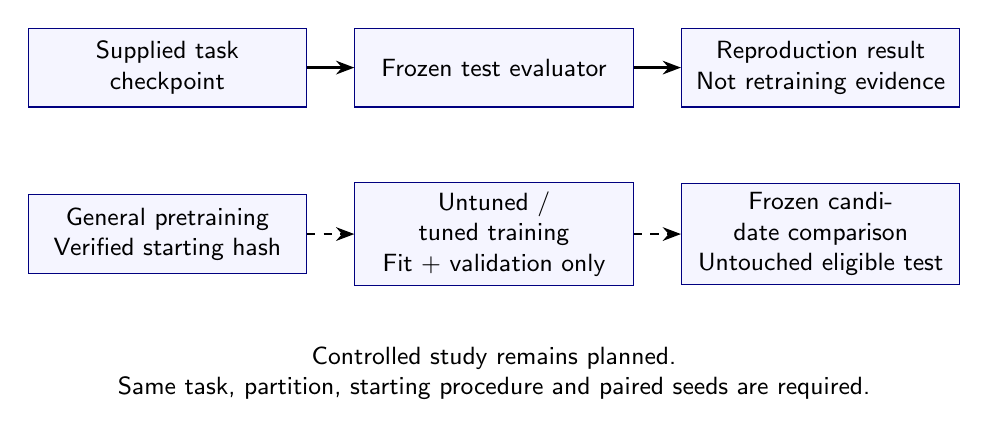
\begin{tikzpicture}[font=\sffamily\small,>=Stealth,
box/.style={draw=blue!50!black,align=center,text width=3.3cm,minimum height=1cm,fill=blue!4}]
\node[box] (a) {Supplied task checkpoint};
\node[box,right=0.6cm of a] (b) {Frozen test evaluator};
\node[box,right=0.6cm of b] (c) {Reproduction result\\Not retraining evidence};
\draw[->,thick] (a)--(b);\draw[->,thick] (b)--(c);
\node[box,below=1.1cm of a] (g) {General pretraining\\Verified starting hash};
\node[box,right=0.6cm of g] (u) {Untuned / tuned training\\Fit + validation only};
\node[box,right=0.6cm of u] (t) {Frozen candidate comparison\\Untouched eligible test};
\draw[->,dashed,thick] (g)--(u);\draw[->,dashed,thick] (u)--(t);
\node[below=0.65cm of u,align=center] {Controlled study remains planned.\\Same task, partition, starting procedure and paired seeds are required.};
\end{tikzpicture}
\end{document}
